% !TeX spellcheck = en_US
\section{DATASET}
\label{sec:dataset}

The dataset provided by the hosts of the competition consists of a training set of 3881 high-resolution images, and a test set of 4150 high-resolution images. No other dataset  has been used. The labels are presented as the unicode encoding of the character to be recognized and the complete annotation (i.e. top, left, bottom, right) of the bounding box that encloses it. A standard image from the dataset is shown in figure \ref{fig:dataset_example}.

\begin{figure}[h]
	\caption{Example of standard image from the dataset.}
	\centering
	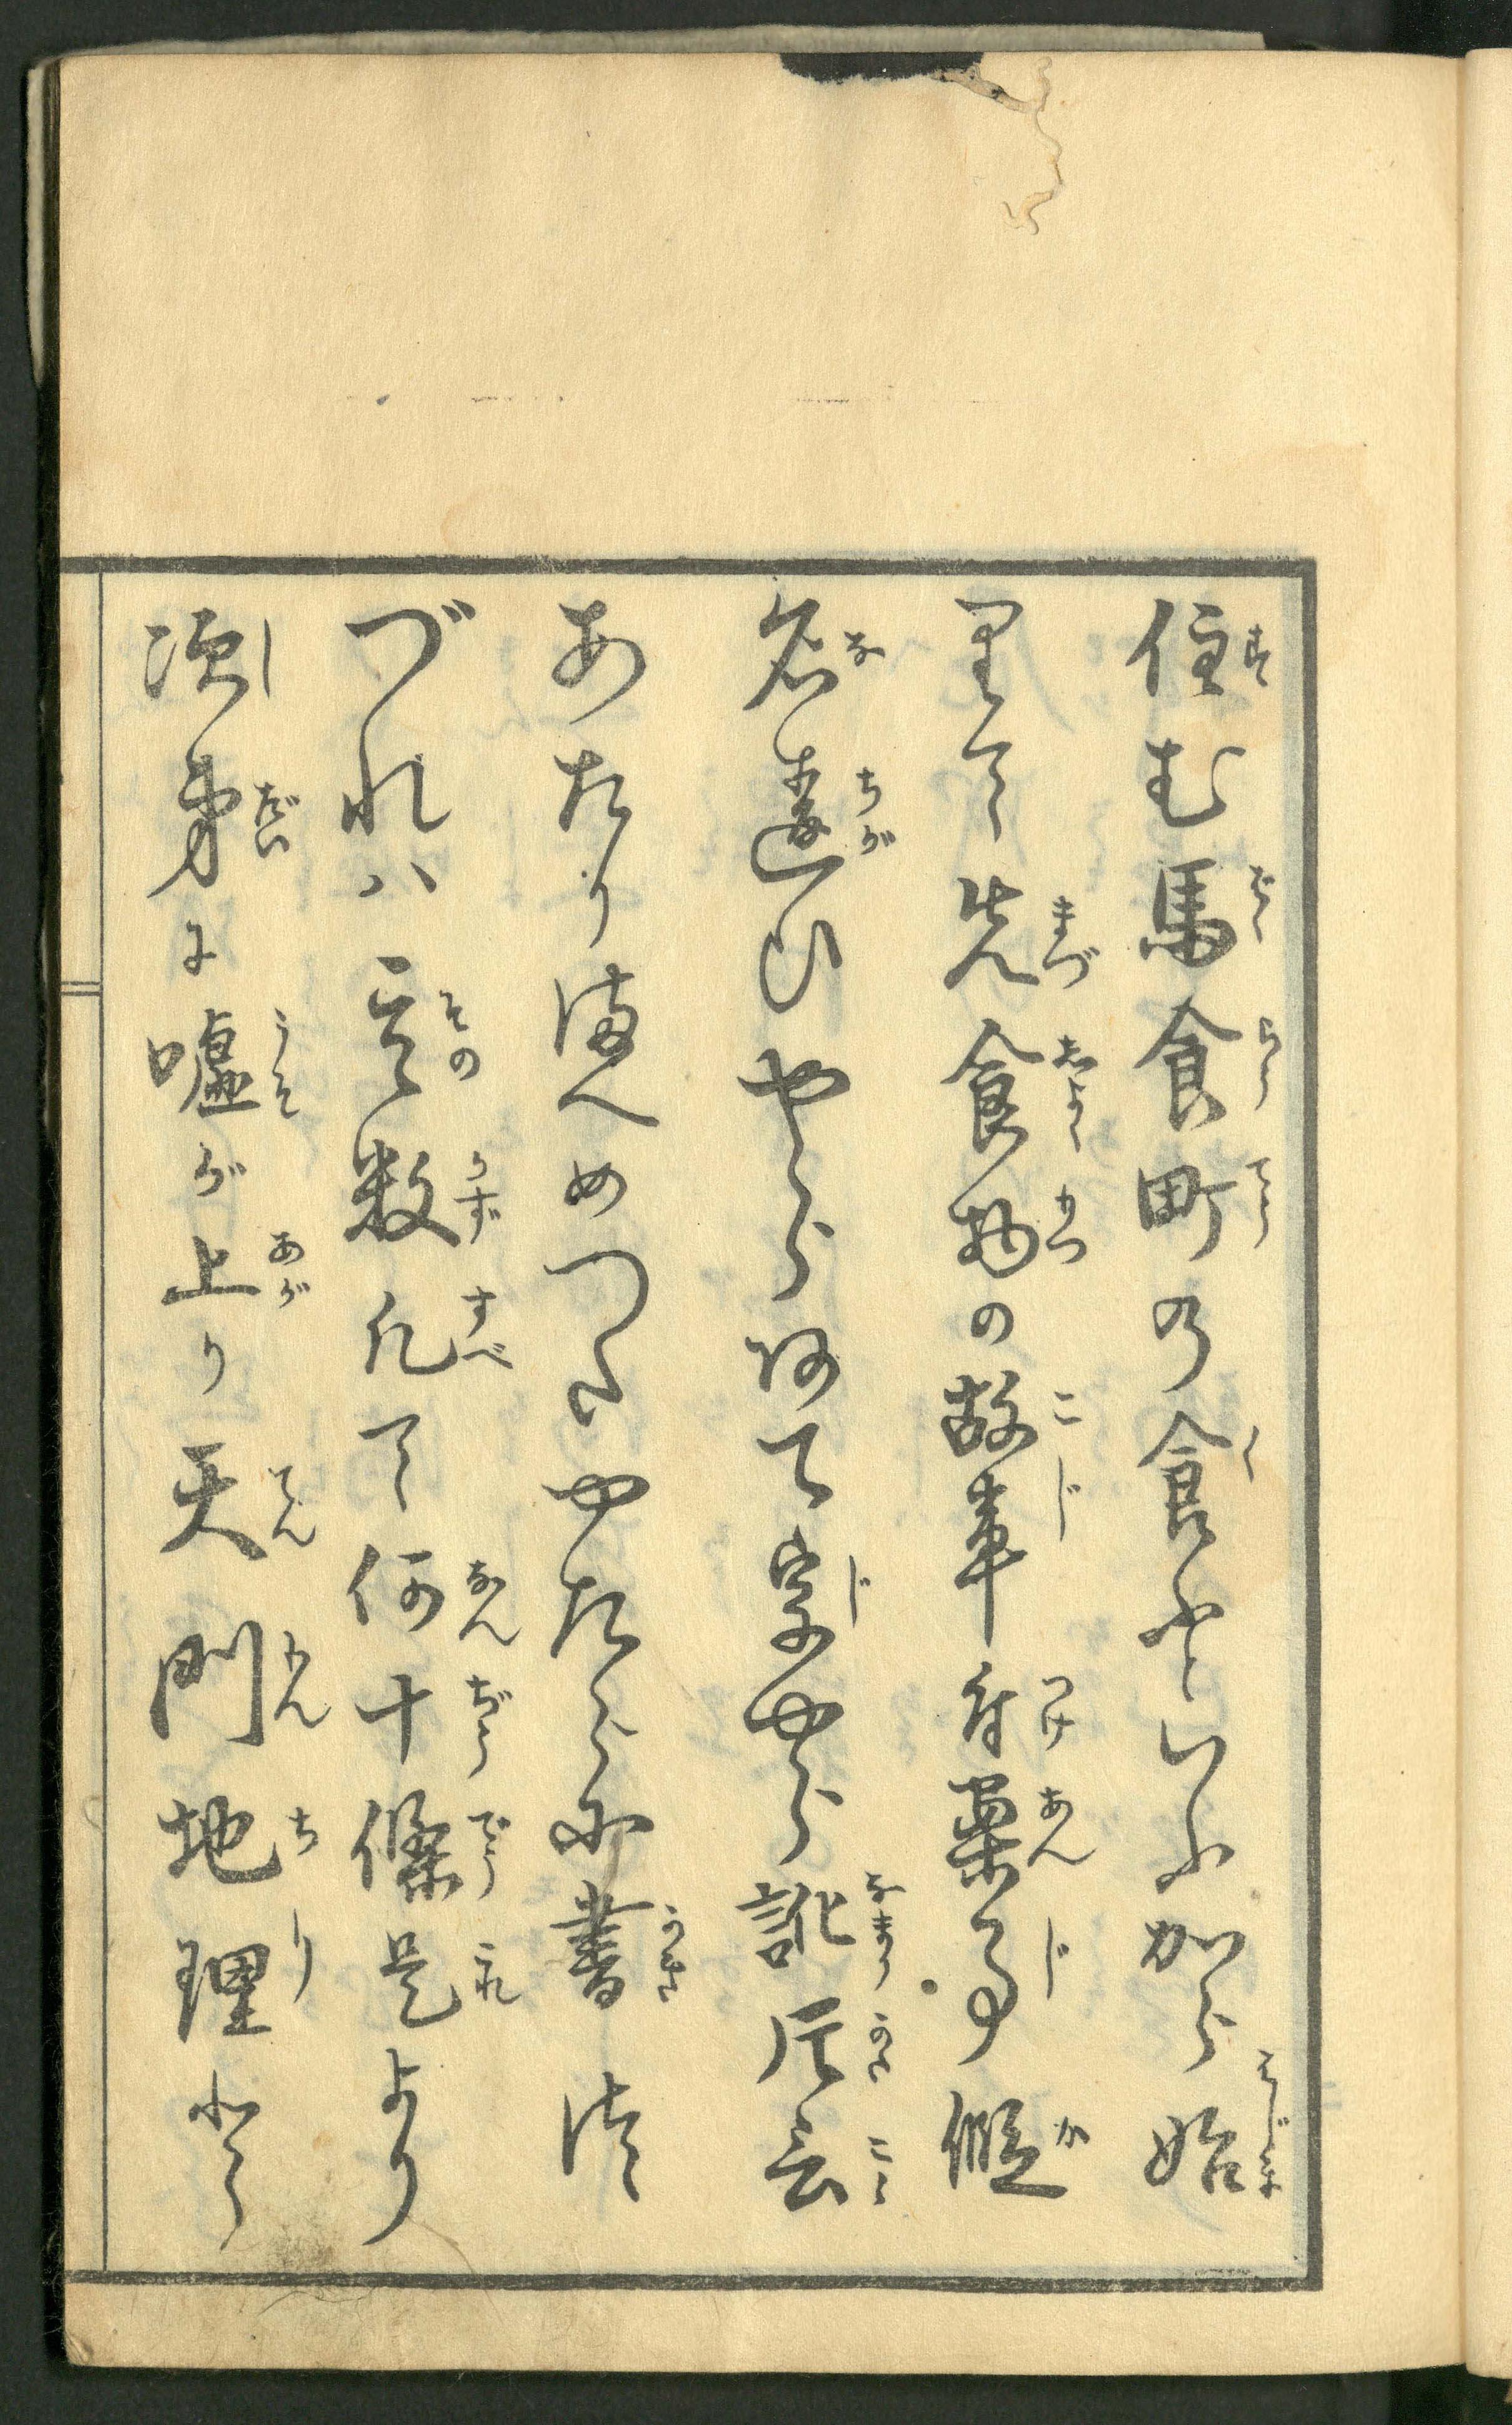
\includegraphics[width=0.3\textwidth]{dataset/dataset_example.jpg}
	\label{fig:dataset_example}
\end{figure}
Several peculiarities of Kuzushiji characters have made their automatic recognition notoriously challenging. Of course, being a cursive writing style, in many cases, characters are connected or overlapped. Furthermore, in Kuzushiji documents Kanji, Hiragana and Katakana, three very different kinds of Japanese writing, are all used, possibly in the same page. A peculiar characteristic of one of these kinds of writing, Classical Hiragana, is that many characters which can only be written in a single way in modern Japanese can be written in many different ways in Kuzushiji, generating multiple orthographic variations of the same character. Besides, a few characters in Kuzushiji also look very similar, making it quite hard to tell what character it is without considering the above character within the context, which may be an interesting hook for the application of a language model. However, the layout of Kuzushiji characters (while normally arranged into columns) does not follow a single simple rule, so it is not always trivial to express the characters as a sequence. The data analysis also brought out some interesting facts about the dataset. First of all, only 4212 out of the possible 4787 Kuzushiji characters are present within the training set. Despite the total number of unique characters in the dataset being quite high, the frequency distribution is very long-tailed and a large fraction of the characters (Kanji with very specific meaning) may only appear once or twice in a book. Therefore, the dataset is highly unbalanced. Some images, like the one in figure ??, also contain illustrations only, in which case no character should be detected. In a similar fashion, the thin paper of the manuscripts sometimes lets characters of the following page transpire. Those characters should be ignored and may score some false positives.
